
\documentclass{article}

% if you need to pass options to natbib, use, e.g.:
%     \PassOptionsToPackage{numbers, compress}{natbib}
% before loading neurips_2018

% ready for submission
% \usepackage{neurips_2018}

% to compile a preprint version, e.g., for submission to arXiv, add add the
% [preprint] option:
\usepackage[preprint]{neurips_2019}

% to compile a camera-ready version, add the [final] option, e.g.:
     % \usepackage[final]{neurips_2019}

% to avoid loading the natbib package, add option nonatbib:
%     \usepackage[nonatbib]{neurips_2018}

\usepackage[utf8]{inputenc} % allow utf-8 input
\usepackage[T1]{fontenc}    % use 8-bit T1 fonts
\usepackage{hyperref}       % hyperlinks
\usepackage{url}            % simple URL typesetting
\usepackage{graphicx}
\usepackage{booktabs}       % professional-quality tables
\usepackage{amsfonts}       % blackboard math symbols
\usepackage{nicefrac}       % compact symbols for 1/2, etc.
\usepackage{microtype}      % microtypography
\usepackage{listings}
\usepackage{tabularx}
\usepackage{listings}
\usepackage{pgfplots}
\usepackage{tikz,pgf}
\usepackage{todonotes}
\usepackage{tikz-cd}
\usepackage{algorithm}
\usepackage{algpseudocode}
\usepackage{wrapfig}
\usepackage{amsmath}

\usetikzlibrary{arrows,automata}
\usetikzlibrary{positioning}
\newcommand{\n}[1]{\ensuremath{n_{#1}}}
\newcommand{\rv}[1]{\ensuremath{{#1}_{1:n_{#1}}}}
\newcommand{\rvv}[1]{\ensuremath{{#1}_{1:n_{#1'}}}}
\newcommand{\model}[1]{\ensuremath{\mathcal{M}{(#1)}}}
\newcommand{\simu}[1]{\ensuremath{\Omega(\model{#1})}}
\newcommand{\micro}[2]{\ensuremath{\phi_{#1}(#2)}}
\newcommand{\pdf}[1]{\ensuremath{\mathcal{P}_{d}(#1)}}
\newcommand{\pmf}[1]{\ensuremath{\mathcal{P}_{m}(#1)}}
\newcommand{\add}[1]{\ensuremath{A_{#1}}}
\newcommand{\adds}[2]{\ensuremath{A_{#1}_{#2}}}
\newcommand{\expect}[1]{\ensuremath{\mathbb{E}[#1]}}
\newcommand{\trace}[1]{\ensuremath{\mathcal{T}_{#1}}}
\newcommand{\traces}[2]{\ensuremath{\textit{tr}^{#1}_{#2}}}
\newcommand{\stoc}[2]{\ensuremath{f^{#1}_{#2}(\rvv{x})}}
% \usepackage[binary-units=true]{siunitx}
\title{Hijacking Simulators with Universal Probabilistic Programming}

% neurlps classification
% Primary: Applications
% Secodnary cat:Data, Challenges, Implementations, and Software
% or Hijacking Malaria Simulators with Probabilistic Programming

% The \author macro works with any number of authors. There are two commands
% used to separate the names and addresses of multiple authors: \And and \AND.
%
% Using \And between authors leaves it to LaTeX to determine where to break the
% lines. Using \AND forces a line break at that point. So, if LaTeX puts 3 of 4
% authors names on the first line, and the last on the second line, try using
% \AND instead of \And before the third author name.
\newcommand{\bg}[1]{~{{[{\it \textcolor{red}{{\bf BG:} #1}}]}}}
\newcommand{\cs}[1]{~{{[{\it \textcolor{red}{{\bf CS:} #1}}]}}}
\newcommand{\ag}[1]{~{{[{\it \textcolor{red}{{\bf AG:} #1}}]}}}
% If accepted, instead use the following line for the camera-ready submission:
%\usepackage[accepted]{icml2019}

\lstset{language=C++,
                basicstyle=\footnotesize,
                keywordstyle=\color{blue}\ttfamily,
                stringstyle=\color{red}\ttfamily,
                commentstyle=\color{green}\ttfamily,
                morecomment=[l][\color{magenta}]{\#},
                breaklines = true
}
\pgfplotsset{width=7cm,compat=1.8}
\author{%
Paper ID: 1010 }
  % examples of more authors
  % \And
  % Coauthor \\
  % Affiliation \\
  % Address \\
  % \texttt{email} \\
  % \AND
  % Coauthor \\
  % Affiliation \\
  % Address \\
  % \texttt{email} \\
  % \And
  % Coauthor \\
  % Affiliation \\
  % Address \\
  % \texttt{email} \\
  % \And
  % Coauthor \\
  % Affiliation \\
  % Address \\
  % \texttt{email} \\
%}
\begin{document}
% \nipsfinalcopy is no longer used

\maketitle

\begin{abstract}

    Notes on how to develop a formalism to perform inference in population based simulators.
\end{abstract}

\section{Introduction}
\label{sec:intro}

One challenge in performing inference in such models is the combinatorial increase in \emph{paths}
that can be taken within the given probabilistic model.
This is because each member of the population has 
a bounded, but large number of decisions to make. 
In addition to this, each member of the population can interact
with other members of the population.
To model a single population member quantum-based methods leveraging 
linear superposition and entanglement provide an ability to explore multiple paths simultaneously maintaining 
the whole program, \emph{state}, in one iteration.
 Unfortunately, analytically writing the functional 
form of the state is, in this instance, impossible.   
The usability of current classical inference methods in this context is also problematic. 
However, by combining hijacking and amortizing parts of the simulator, in particular rejection sampling 
loops, we can not only correctly perform inference in such models, as the rejection sampling loops are 
now replaced with learnt functions, but we can also perform inference much more efficiently. 
This is because the rejection sampling loops are now replaced with learnt functions which enables us to correctly
construct the density and as they are amortized evaluation is cheap and only has to be performed once per call.
This both reduces memory consumption and running time. 

As updates are made sequentially MCMC methods typically are not-well suited this type of recursive
estimation problem. 
As each time we get a new data point $y_{t+1}$ we have to run new MCMC simulations 
for $P(x_{0:t_1}| y_{0:t+1})$, we also cannot directly reuse the samples $\{x^{i}_{0:t}\}$. 
Likewise, importance sampling is not well suited either, as we cannot reuse the samples and weights for a time $t$ $\{x^{i}_{0:t}, \tilde{w}^{i}_{t}\}^{N}_{i=1}$ 
to sample from $(x_{0:t_1}| y_{0:t+1})$.
 However, as we can only run the simulator $\texttt{forward()}$ we cannot return back to a previous state and re-run. So adapting existing inference techniques 
 is the only viable option. 

 % !TEX root = notes.tex

\tikzset{
    state/.style={
           rectangle,
           rounded corners,
           draw=black, very thick,
           minimum height=2em,
           inner sep=2pt,
           text centered,
           },
}

\begin{figure}
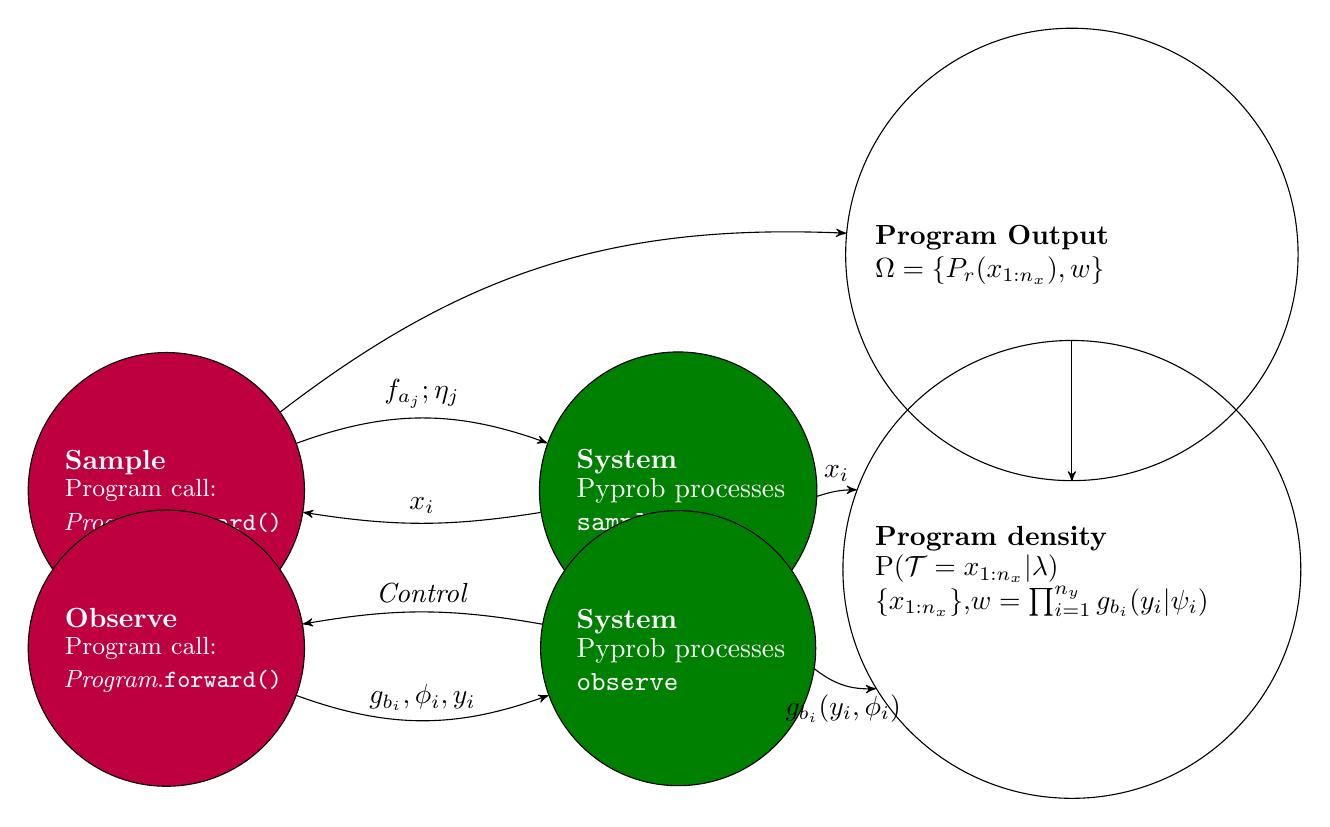
\begin{tikzpicture}[->,>=stealth']

 % Position of Sample 
 % Use previously defined 'state' as layout (see above)
 % use tabular for content to get columns/rows
 % parbox to limit width of the listing
 \node[state,
 text width=3cm, 	% max text width
 yshift=0cm, 		% move 2cm in y
 node distance=0cm, 	% distance to Sample
 anchor=center,
 fill=purple] (Sample) 
{%
\begin{tabular}{l} 	% content
  \textcolor{white}{\textbf{Sample}}\\
  \parbox{4cm}{
  \textcolor{white}{\small{Program call:\\
  \emph{Program}.\texttt{forward()}}}
 }
 \end{tabular}};
  
 \node[state,    	% layout (defined above)
 text width=3cm, 	% max text width
 yshift=-2cm, 		% move 2cm in y
 below of=Sample, 	% Position is to the right of Sample
 node distance=0cm, 	% distance to Sample
 anchor=center,
 fill= purple] (OBSERVE) 	% posistion relative to the center of the 'box'
{%
\begin{tabular}{l} 	% content
  \textcolor{white}{\textbf{Observe}}\\
 \parbox{4cm}{
  \textcolor{white}{\small{Program call:\\
  \emph{Program}.\texttt{forward()}}}
}
\end{tabular}};

 % State: PyProb with different content
 \node[state,    	% layout (defined above)
  text width=3cm, 	% max text width
  yshift=0cm, 		% move 2cm in y
  right of=Sample, 	% Position is to the right of Sample
  node distance=6.5cm, 	% distance to Sample
  anchor=center,
  fill = black!50!green] (PyProb) 	% posistion relative to the center of the 'box'
 {%
 \begin{tabular}{l} 	% content
  \textcolor{white}{\textbf{System}}\\ %system sample
  \parbox{4cm}{\textcolor{white}{Pyprob processes\\ \texttt{sample}}}
 \end{tabular}
 };
 
 % STATE System
 \node[state,
  below of=PyProb,
  yshift=-1cm,
  anchor=center,
  text width=3cm,
  fill = black!50!green] (System) 
 {%
 \begin{tabular}{l}
  \textcolor{white}{\textbf{System}}\\
  \parbox{4cm}{\textcolor{white}{Pyprob processes \\\texttt{observe}}}
 \end{tabular}
 };

 % STATE EPC
 \node[state,
  right of=System,
  yshift = 1cm,
  node distance=5cm,
  anchor=center] (EPC) 
 {%
 \begin{tabular}{l}
  \textbf{Program density}\\
  \parbox{5cm}{P($\mathcal{T}= x_{1:n_x}| \lambda)$\\
  \{$x_{1:n_{x}}\}$,$w= \prod^{n_{y}}_{i=1} g_{b_i}(y_i | \psi_i)$}
 \end{tabular}
 };


  % STATE OUTPUT
  \node[state,
  above of=EPC,
  yshift = -1cm,
  node distance=5cm,
  anchor=center] (OUTPUT) 
 {%
 \begin{tabular}{l}
  \textbf{Program Output}\\
  \parbox{5cm}{$\Omega = \{P_{r}(x_{1:n_{x}}), w\}$}
 \end{tabular}
 };

 % draw the paths and and print some Text below/above the graph
 \path (Sample) 	edge[bend left=20]  node[anchor=south,above]{$f_{a_{j}} ; \eta_{j}$}(PyProb)
 (OBSERVE)     	edge[bend right=20] node[anchor=south,above]{$g_{b_{i}},\phi_i , y_i $} (System)
 (System)       	edge [bend right=20] node[anchor=south,below]{$g_{b_{i}}(y_i, \phi_i)$} (EPC)
 (PyProb)       edge [bend left=9] node[anchor=west, above]{$x_{i}$} (Sample)
 (PyProb)       edge [bend left=9] node[anchor=west, above]{$x_{i}$} (EPC)
%  (System)       	edge [bend left=10]                                          (EPC)
 (EPC)              edge                                                    (OUTPUT)
 (System)  	edge [bend right=10]  node[anchor=north,above]{\emph{Control}} (OBSERVE)
 (Sample)   edge [bend left= 20] (OUTPUT) ;
%  (System)  	edge[loop below]    node[anchor=north,below]{$SC_n\neq 0$} (System)
%  (System)  	edge                node[anchor=left,right]{$SC_n = 0$} (PyProb);

\end{tikzpicture}
\caption{An overview of the hijacking system. $x_i$ represent latent variables. $f_{a_i}$ represent raw sample calls,
$g_{b_j}$ represent conditioning statements. $\mathcal{T}$ corresponds to the program trace. $w$ represents the collective weights. 
$r$ represents run number. $n_x$ represents the number of latent variables and $n_y$ represents the number of
observations, which will always be fixed, but is model dependent. $\lambda$ represents all the other variables generated 
by running the simulator \texttt{.forward()}.
}
\label{fig:systemoverview}
\end{figure}
\section{Limitations with different inference engines}  

\subsection{Prior based sampling}
In prior based sampling we take our existing program and look directly at the product of all the raw sample calls, denoted $f_{a_i}(x_i | \eta)$ and 
construct a proposal that is is dependent on those. In this sampling scheme our proposal is defined as:
\begin{equation}
  q(x_{1:n_{x}}) = 
  \begin{cases}
    \prod_{j=1}^{n_x} f_{a_i}(x_i | \eta) \hspace{0.1cm} \texttt{if} \hspace{0.1cm} \mathcal{B}(x_{1:n_{x})=1 \\
    0
  \end{cases}
\end{equation}
However, this makes use of no conditioning and is not sufficient for performing inference in
complex, population-based simulations.

\section{Non-prior Based Sampling}

\subsection{Importance Sampling}

\subsection{Sequential Monte Carlo}

\subsection{Random-walk Metropolis Hastings}

\bibliographystyle{plain}
\bibliography{refs}

\end{document}